\subsection{Salt Rock Samples}
\label{subsec:salt}
\Authors{IfG}

\subsubsection{The Springen in-situ laboratory}
\label{sec:springen}
\todo[inline]{[IfG](): Introduction to Springen in-situ laboratory}

\subsubsection{Rock salt laboratory}

The following conditions and equipment are available in the IfG labs for rock mechanical laboratory investigations:

\begin{list}{-}{\leftmargin=1em \itemindent=0em \itemsep=0.1em}
\item Climate-controlled rooms for storage of specimens at conditions which correspond to those present in situ
\item Laboratory for mineral-petrographic examinations, density and moisture determination, ultra-sound measurements and 
photographic documentation
\item Workshop for the preparation of specimens in high precision according to testing requirements (rock saws, lathes etc.)
\item Test laboratory containing various servo-controlled hydraulic testing machines for conducting investigations on 
rock mechanics in accordance with the up-to-date state of research and development (see Figure \ref{fig:ifglabph1}).
\end{list} 

\begin{figure}[!ht]
\centering
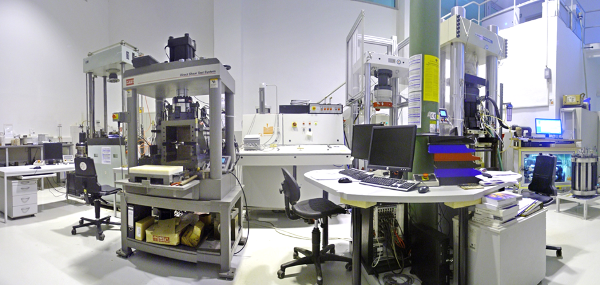
\includegraphics[width=1\textwidth]{./figures/ifg-lab-photo1-v2.png}
\caption{View inside the rock mechanical lab with various servo-controlled hydraulic testing machines.}
\label{fig:ifglabph1}
\end{figure}

It has to be mentioned that some of the applied IfG test procedures have been developed for the requirements of the specific IfG-material laws. 
But generally they are in accordance to ASTM and ISRM standards resp. equivalent descriptions, e.g.:

\begin{list}{-}{\leftmargin=1em \itemindent=0em \itemsep=0.1em}
\item ASTM D 4543-85 Standard Practice for Preparing Rock Core Specimens and Determining Dimensional and Shape Tolerances
\item ASTM D 2845-05 Standard Test Method for Laboratory Determination of Pulse Velocities and Ultrasonic Elastic Constants of Rock
\item ASTM D 2664-86 Standard Test for Triaxial Compressive Strength of Undrained Rock Core Specimens without Pore Pressure Measurements 
\item DGEG (1979):   Empfehlung Nr. 2 des AK 19 der DGEG (Dreiaxiale Druckversuche).
\item ASTM D4406-04 Standard Test Method for Creep of Cylindrical Rock Core Specimens in Triaxial Compression
\item ASTM D7070-04 Standard Test Method for Creep of Rock Core Under Constant Stress and Temperature
\item ISRM: Suggested Methods for Determining o the Uniaxial Compressive Strength and Deformability of Rock Materials
\item ISRM: Suggested Methods : Part 2 : 2007 - Unconfined Compressive Strength with Young's Modulus and Poisson's Ratio
\item ISRM: - Suggested Methods : Part 2 : Received 1983 - Strength of Rock Material in Triaxial Compression
\end{list}

\subsubsection{Sample characterization and pre-investigation}

Several preliminary investigations are usually done before lab testing. After preparing the cylindric samples (cutting with a rock saw and smoothing the samples with a lathe) in the IfG labs, their density is determined by measuring the geometrical dimensions and the mass. Concerning the quality of these parameters an accuracy in length determination is $<$ 0.01 mm, those in mass determination is $<$ 0.01 g. 

Additionally, ultrasonic investigations are carried out to check integrity, homogeneity and isotropy of the samples. The ultrasonic pulse measurement system used for transmission of the rock specimens consists of two transducer sets for P-waves and S-waves and a receiver system for generating and evaluating the ultrasonic signals. The specimen is placed in physical contact between two piezoelectric transducers, one acts as a driver and the other one acts as a receiver. The transit time of the mechanical pulse to pass through the specimen is used to determine elastic wave velocity.

For samples where both P- and S-waves were measured in axial sample direction the elastic constants are obtained from density ($\rho$) and the ultrasonic velocities ($v_p$, $v_s$) using the following expressions derived from the theory of elasticity for homogeneous, isotropic solids:

\begin{equation}
\label{eq:YoungsModulus_Ultrasonic}
E_{dyn} = \frac{\rho v_s^2(3v_p^2-4v_s^2)}{v_p^2-v_s^2} 
\end{equation}
\begin{equation}
\label{eq:PoissonsRatio_Ultrasonic}
\nu_{dyn} = \frac{v_p^2-2v_s^2}{2(v_p^2-v_s^2)}
\end{equation}

Dynamic elastic parameters of the various rock portions determined on the base of sonic wave velocity at room temperature are in a wide range representing typical values for the various materials as known from other locations. 

\subsubsection{Triaxial compression strength tests (TC) - methodology and equipment}
\index{triaxial compression test (TC)}
\todo{[IfG]() This section could be shifted to section \ref{sec:thm-lab-tests}?}

Triaxial compression tests (TC) are executed on cylindrical core samples with dimensions of e.g. 200*100 mm (generally a 2:1 ratio of height to diameter) in one of two available servo-hydraulic testing machines of the IfG labs (RBA 2500, Schenk/Trebel, Germany and D2000 GGL Testsystems – using the MTS-TestStar software; see Fig. \ref{fig:ifglabph2} generating the necessary stress $\sigma_1$ in axial direction and $\sigma_3$ in lateral direction.

The cylindrical samples are sealed with rubber tubes and oil is used as confining medium. Outside the vessel three LVDT transducers are mounted between the piston and the load frame near the sample for the measurement of the axial strain. The axial load is determined from an external load cell. Tests can also be carried out at in-situ relevant temperatures (e.g. 55$^\circ$C). During all tests the following parameters are measured automatically: the axial deformation $\Delta h$, axial load $F$ and the confining pressure $p = \sigma_3$. The conversion of the measured values to effective stress and strain is given as:

\begin{equation}
\sigma_{eff} = \left(  \frac{F}{A_0}-\sigma_3 \right) (1-\epsilon_1)
\end{equation}
\begin{equation}
\epsilon_1 = \frac{h_0-h}{h_0}
\end{equation}
with
\begin{tabbing}
symbo \= description \kill
$h_0$, $h$ : \> length of the sample before and during deformation \\
$A_0$ : \> cross sectional area of the undeformed sample \\
$F$ : \> axial load  \\
$\sigma_3$ : \> confining pressure 
\end{tabbing}

The term $1-\epsilon_1$ results from the consideration of the sample bulge during the deformation, e.g. the changes of the cross sectional area as well in compression as in extension are regarded.

In addition, as a standard technique of the IfG during the triaxial strength experiments the sample volume changes $\Delta V$ are determined by a volume balance of the mantle oil volume changes as measured via the pressure intensifier and the axial piston displacement in the cell:

\begin{equation}
\Delta V = \Delta h A_{pp} -\Delta S_{pi} A_{pi}
\end{equation}
with
\begin{tabbing}
symbo \= description \kill
$\Delta h$ : \> displacement of the piston of the triaxial cell \\
$A_{pp}$ : \> cross section of the piston of the triaxial cell \\
$\Delta S_{pi}$ : \> displacement of the cylinder within the pressure intensifier \\
$A_{pi}$ : \> cross section of the piston within the pressure intensifier \\
\end{tabbing}

During all tests the following parameters were measured automatically: The axial deformation $\Delta h$, axial load $F$ and the confining pressure $p = \sigma_3$. 

The triaxial test procedure is divided into two steps:

\begin{list}{-}{\leftmargin=1em \itemindent=0em \itemsep=0.2em}
\item 1st step: Reconsolidation – isotropic phase (applied for all samples): Because it is assumed that core material is generally dilated due the applied procedures during core recovery (stress relaxation) and subsequent weathering, the samples are firstly re-compacted. In a hydrostatic load cycle ($\sigma_1 = \sigma_3$) the samples are pressurized up to 60 MPa (at 0.01 MPa/s) and then, after 30 min. unloaded to the respective pressure state of the strength test.
\item 2nd step: Triaxial test cycle – deviatoric phase:  At constant confining pressure the sample is axially loaded using a constant deformation rate, until the sample fails and reaches the post failure state. Common standard triaxial compression tests (TC) with defined deformation rate at constant confining pressures are between 1 and 25 MPa. A determination of the deformation dependent strength and dilatancy behavior is realized, too.
\end{list}
\index{dilatancy}

The standard triaxial strength test (TC) for salt rocks is performed with a constant deformation rate 
(5$\cdot$10$^{-6}$ s$^{-1}$) at constant confining pressure. After the failure occurs the axial load decreases with further deformation due to the decrease of the load-bearing capacity becoming nearly constant if the post-failure stage is reached. Finally the sample is unloaded.

Simultaneously with the deformation the volumetric strain is measured which allows to determine the 
stress-dependent onset of micro-cracking (given by the minimum) and to quantify the deformation induced damage.

\begin{figure}[!ht]
\centering
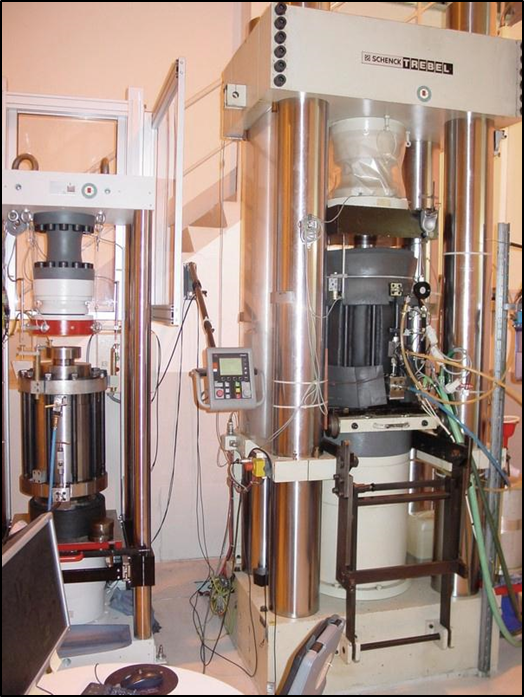
\includegraphics[width=1\textwidth]{./figures/ifg-lab-photo3.png}
\caption{The two available servo-controlled hydraulic testing machines (right: system RBA 2500 of SCHENK/TREBEL and left: D2000 of GGL TestSystems)}.
\label{fig:ifglabph2}
\end{figure}